\section{氢气的实验室制法}\label{sec:2-2}

早在十六世纪的时候,人们就知道,把稀硫酸倒在某些金属上,
会产生一种可燃性气体,当时人们就叫这种气体为 “可燃性空气”。
直到十八世纪中期,人们才知道,这种气体根本不是空气,而是一种新的物质。
它就是氢元素组成的单质——氢气。氢气是最轻的气体,因此,人们把它命名为 “氢”。

直到现在,实验室里还用稀硫酸跟金属起反应来制取氢气。金属通常使用的是锌粒。

\begin{wrapfigure}[8]{r}{5cm}
    \centering
    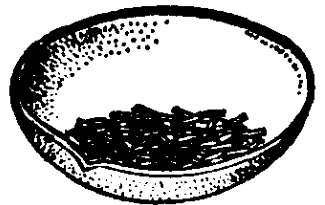
\includegraphics[width=4cm]{../pic/czhx1-ch2-2}
    \caption{溶液蒸发后析出硫酸锌}\label{fig:2-2}
\end{wrapfigure}

\wrapfiguretrick

\begin{shiyan}
    在试管里放几粒锌粒,加 $5$ 毫升稀硫酸,用燃着的木条放在管口,观察发生的现象。
    等到反应完毕,把试管里的液体倒入蒸发皿里,小心加热,使液体蒸发。
    冷却后在蒸发皿里可以看到什么物质?
\end{shiyan}

从上面的实验可以看到,锌跟稀硫酸起反应放出的氢气,点火发生燃烧。
另外,液体经蒸发冷却后,蒸发皿里留下无色的固态物质(图 \ref{fig:2-2})。
这种物质叫做硫酸锌(\ce{ZnSO4})。因此,这个反应可以用化学方程式表示如下:
\begin{fangchengshi}
    \ce{ $\underset{\text{锌}}{\ce{Zn}}$
        +
        $\underset{\text{硫酸}}{\ce{H2SO4}}$
        =
        $\underset{\text{硫酸锌}}{\ce{ZnSO4}}$
        +
        $\underset{\text{氢气}}{\ce{H2 ^}}$
    }
\end{fangchengshi}

也可以用盐酸代替硫酸,用镁或铁代替锌,来制取氢气。
反应的结果同锌跟稀硫酸的反应类似,除生成氢气外,同时各生成另一种物质。
这两个反应的化学方程式分别是:

\begin{fangchengshi}
    \ce{ $\underset{\text{镁}}{\ce{Mg}}$
        +
        2 $\underset{\text{盐酸}}{\ce{HCl}}$
        =
        $\underset{\text{氯化镁}}{\ce{MgCl2}}$
        + H2 ^
    } \\
    \ce{ $\underset{\text{铁}}{\ce{Fe}}$
        + 2 HCl =
        $\underset{\text{氯化亚铁}}{\ce{FeCl2}}$
        + H2 ^
    }
\end{fangchengshi}

上面三个反应跟分解反应和化合反应不同,它们都是%
\zhongdian{由一种单质跟一种化合物起反应,生成另一种单质和另一种化合物,这类反应叫做置换反应。}

硫酸分子里由一个硫原子和四个氧原子结合而成的 \ce{SO4} 部分,在反应前后没有变化,
只是在反应以前跟氢原子结合,反应以后跟锌原子结合。
通常把硫酸分子里的 \ce{SO4} 部分叫做硫酸根。
它在许多化学反应里,作为一个整体参加反应,好象一个原子一样。
这样的原子集团,叫做\zhongdian{原子团}。
如硝酸铵 \ce{NH4NO3} 中的铵根 \ce{NH4} 和硝酸根 \ce{NO3},
氯酸钾 \ce{KClO3} 中的氯酸根 \ce{ClO3},
高锰酸钾 \ce{KMnO4} 中的高锰酸根 \ce{MnO4},
氢氧化钙 \ce{Ca(OH)2} 中的氢氧根 \ce{OH},都是原子团。

\begin{figure}[htbp]
    \centering
    \begin{minipage}[b]{7cm}
        \centering
        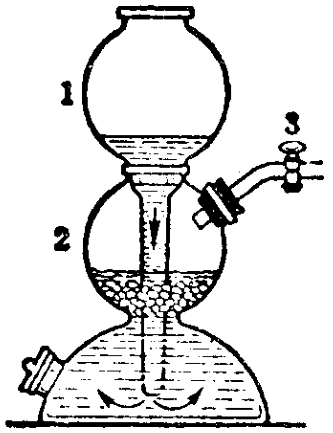
\includegraphics[width=4cm]{../pic/czhx1-ch2-3-1}
        \caption*{I. 扭开活塞时的情形}
    \end{minipage}
    \qquad
    \begin{minipage}[b]{7cm}
        \centering
        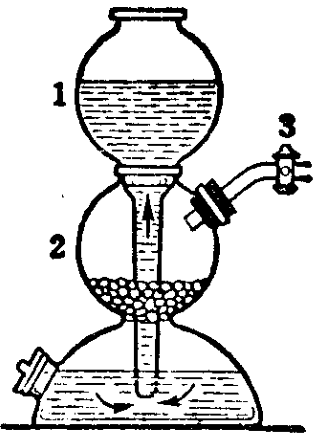
\includegraphics[width=4cm]{../pic/czhx1-ch2-3-2}
        \caption*{II. 关闭活塞时的情形}
    \end{minipage}
    \caption{启普发生器}\label{fig:2-3}
\end{figure}

实验室里制取氢气的装置常用启普发生器\footnote{启普(Kipp,1806 —\, 1864),
荷兰化学家。这种制取气体的发生器是启普设计的,因此以他的名字命名。}。
启普发生器(图 \ref{fig:2-3}) 由球形漏斗 1 、容器 2 和导气管 3 三部分组成。
锌粒由插导气管的口子加入,稀硫酸(或盐酸)由球形漏斗加入。
使用时扭开导气管活塞,酸液从球形漏斗流下,浸没锌粒,发生反应,产生的氢气从导气管
放出\footnote{最初使用时,先要把启普发生器里原有的空气排出,然后使用放出的氢气。}。
不用时关闭导气管活塞,容器内氢气压力加大,把酸液压回球形漏斗里,使酸与锌粒脱离接触,反应即自行停止。
用启普发生器制取氢气,可以随时使反应发生,也可以随时使反应停止,使用起来很方便。
凡利用块状固体跟液体起反应制取气体,只要反应不需加热而且生成的气体难溶于水,就可应用这种仪器。


\begin{figure}[htbp]
    \centering
    \begin{minipage}[b]{7cm}
        \centering
        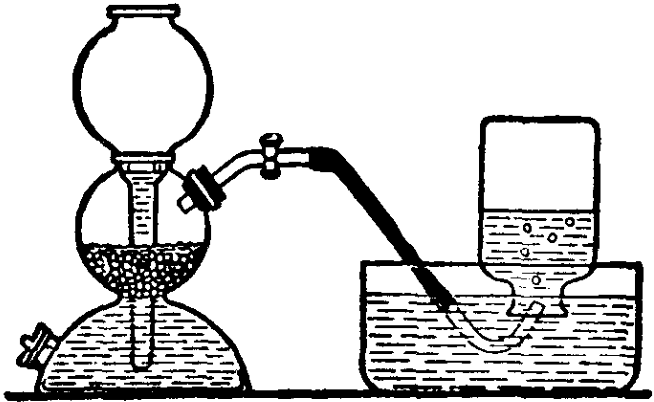
\includegraphics[width=6cm]{../pic/czhx1-ch2-4}
        \caption{用排水法收集氢气}\label{fig:2-4}
    \end{minipage}
    \qquad
    \begin{minipage}[b]{7cm}
        \centering
        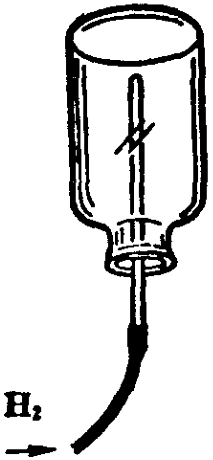
\includegraphics[width=2cm]{../pic/czhx1-ch2-5}
        \caption{用向下排空气法收集氢气}\label{fig:2-5}
    \end{minipage}
\end{figure}


\begin{shiyan}
    分别用排水法和向下排空气法从启普发生器各收集一瓶氢气,
    见图 \ref{fig:2-4}、图 \ref{fig:2-5}。
    为什么收集氢气可分别用这两种方法?
\end{shiyan}


由于氢气难溶于水,所以可用排水法收集;
又由于它比空气轻,所以也可用向下排空气法(容器口朝下)收集。
为了防止氢气散逸,充满氢气的容器也须口朝下倒放。

如果需要氢气的量不多,也可以用图 \ref{fig:2-6} 所示的简易装置来制取。

\begin{figure}[htbp]
    \centering
    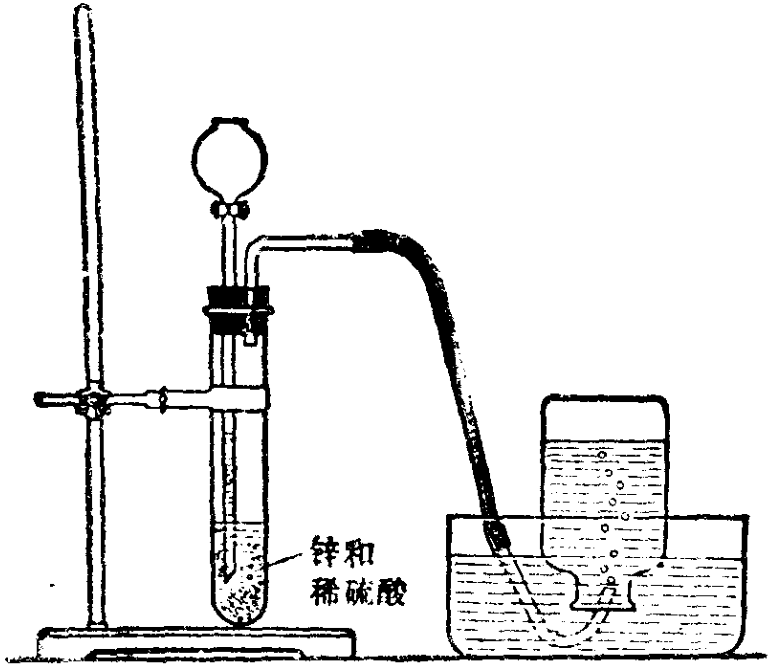
\includegraphics[width=9cm]{../pic/czhx1-ch2-6}
    \caption{制取氢气的简易装置}\label{fig:2-6}
\end{figure}

工业上常用水、水煤气〔主要成分是一氧化碳(\ce{CO})和氢气〕、天然气(主要成分是碳和氢的化合物)等来制备氢气。


\begin{xiti}

\xiaoti{用化学方程式表示实验室制取氢气的反应,并画出制取氢气的简易装置图。
    如用长颈漏斗,为什么长颈漏斗的管囗要插到液面下而不能位于液面上?
    为什么收集氢气可用排水法?用排空气法收集氢气时为什么瓶口要向下?
}

\xiaoti{叙述启普发生器制取氢气的原理。使用启普发生器有什么方便?}


\xiaoti{在下列四个化学反应里,分别指出每个反应是置换反应、分解反应还是化合反应。}
\begin{xiaoxiaotis}

    \xxt{\ce{ S + O2 $\xlongequal{\text{点燃}}$ SO2 }}

    \xxt{\ce{ Fe + H2SO4 =
        $\underset{\text{硫酸亚铁}}{\ce{FeSO4}}$
        + H2 ^
    }}

    \xxt{\ce{ Zn +
        $\underset{\text{硫酸铜}}{\ce{CuSO4}}$
        = Cu + ZnSO4
    }}

    \xxt{\ce{ $\underset{\text{氢氧化铜}}{\ce{Cu(OH)2}}$
        $\xlongequal{\Delta}$
        CuO + H2O
    }}

\end{xiaoxiaotis}


\xiaoti{在下列的物质中,凡含有原子团的,在它的分式相应部位下划一横道,并写出原子团的名称。 \\
    \ce{KClO3},\; \ce{MnO2},\; \ce{KMnO4},\; \ce{Ca(OH)2},\; \ce{P2O5},\; \ce{H2SO4},\; \ce{ZnSO4}, \\
    \ce{NH4Cl}(氯化铵),\; \ce{NH4NO3},\; \ce{(NH4)2SO4}(硫酸铵)。
}

\end{xiti}


